
In a perfect world, experimental and simulated data could be immediately utilized to compute cross-sections once obtained. In reality, a variety of factors - such as defects in experimental detectors or issues in modeling real-world physics - necessitate minor adjustments to be made to the datasets. It is of course not feasible to re-run entire experiments just to address these small issues, and instead is best handled by pre-processing the data with well-motivated correcting factors.  In particular, the experimental data requires fiducial cuts corresponding to detector dead-zones or otherwise problematic areas, as well as energy loss corrections due to underestimates in the reconstruction scheme. The simulated datasets require smearing factors to more closely resemble the real-world detector and reconstruction algorithm performances. 

\subsection{Experimental Data Pre-Processing}
     %\subsubsection{Momentum Corrections}{Mom Corr}
%\subsubsection{Energy Loss Corrections}
Charged particles lose energy via ionization and radiation along their paths. Reconstruction schemes attempt to correct for this, but issues can remain in various situations. The electron reconstruction showed negligible deviations from expected performance. The proton reconstruction exhibited a two-band structure due to detector topology, as shown in \ref{fig:protoncorra}. The issue was deeply studied by S. Lee, who developed and implemented a correction scheme \parencite{Lee2022MeasurementDetector}. We demonstrate in \ref{fig:protoncorrb} the correction is functioning as expected in this work. 


    \begin{figure}[H]
        \centering
        
        \subfloat[Distribution without correction. \label{fig:protoncorra}]{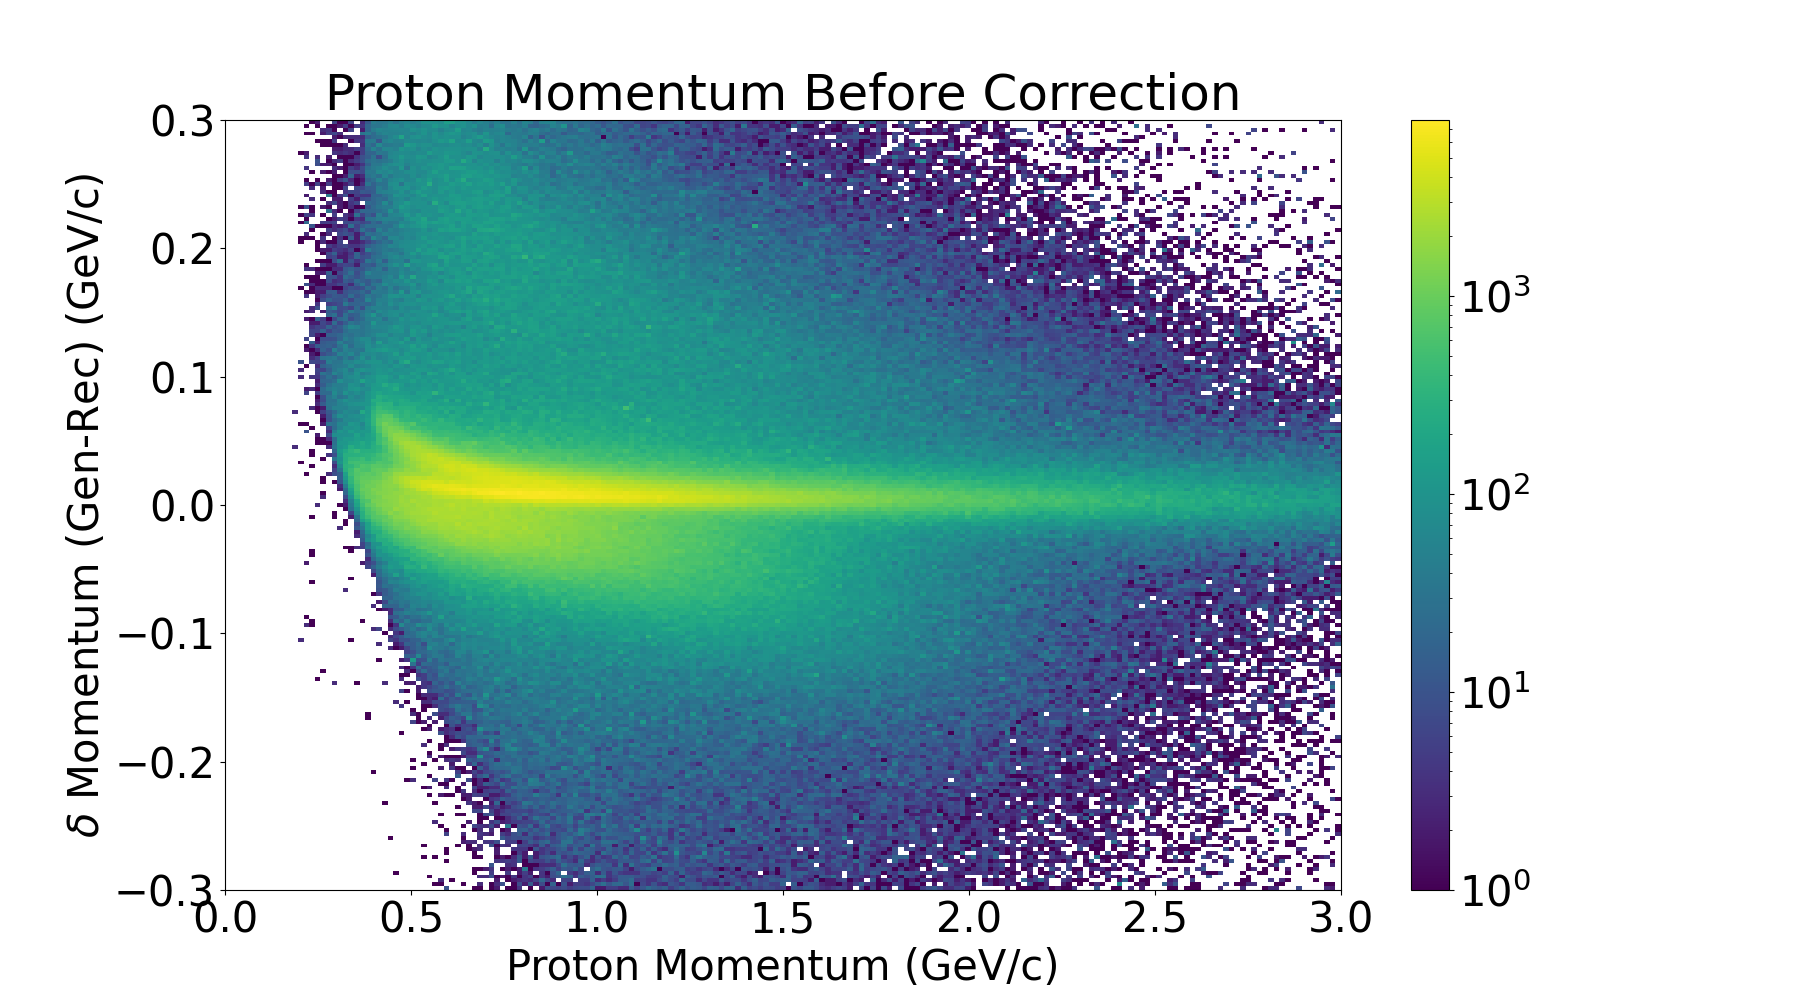
\includegraphics[trim={0 0 5cm 0},clip,width=0.5\textwidth]{Chapters/Ch4-BaseAnalysis/0_preprocessing/0_A_experimental_data_preprocessing/pics/noneProton_Momentum_Before_Correction.png}}
        \hfill
        \subfloat[Distribution with correction. \label{fig:protoncorrb}]{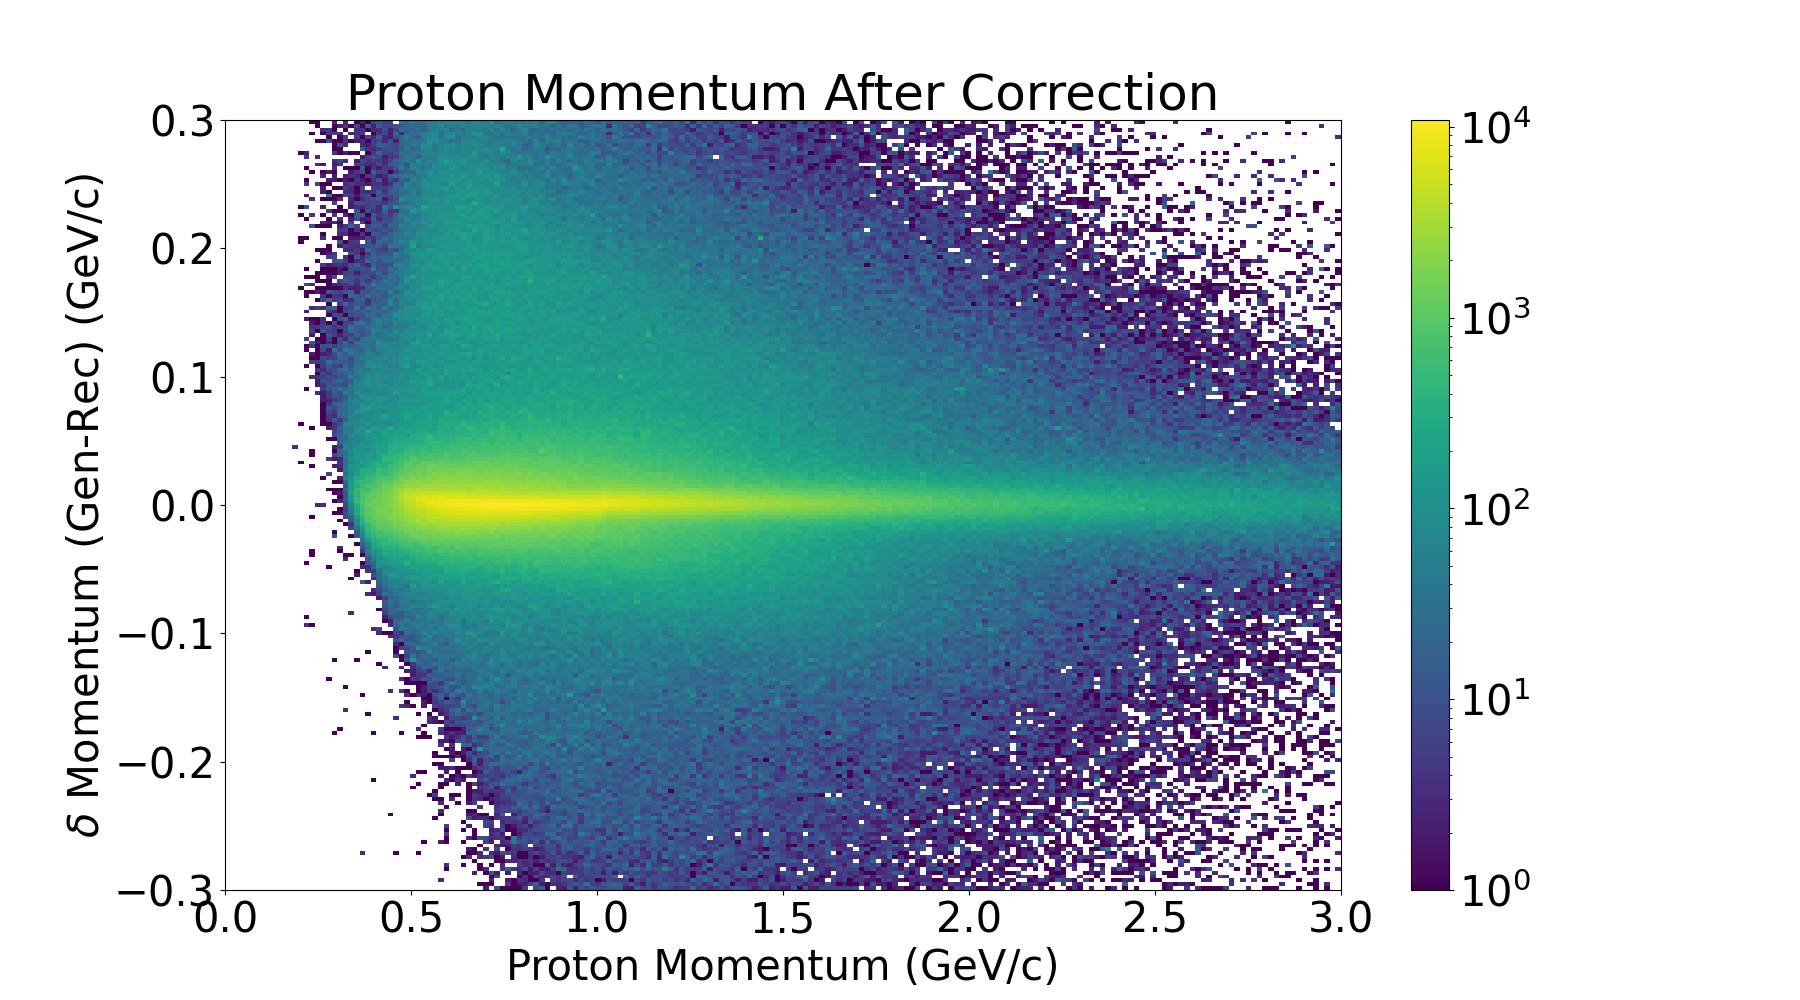
\includegraphics[trim={0 0 5cm 0},clip,width=0.5\textwidth]{Chapters/Ch4-BaseAnalysis/0_preprocessing/0_A_experimental_data_preprocessing/pics/noneProton_Momentum_After_Correction.png}}
    
        \caption[Proton Momentum Correction]{Difference between generated and reconstructed proton momentum as a function of proton momentum, before (a) and after (b) momentum corrections are implemented.}\label{fig:protoncorr}
    \end{figure}

\iffalse
A charged particle loses its energy through its passage through material via ionization
and radiation

We first corrected the energy loss of the proton using the simulation data. After
applying the proton loss corrections to the experimental data and the simulation, we
reduced the reconstruction bias by correcting the single particle kinematics in the
experimental data. To match the resolution, the kinematics of the simulated data
was smeared.

\fi
     
\subsection{Simulation Data Pre-Processing}
   %\subsubsection{Simulation:Experiment Resolution Matching}

The detector responses in the GEMC system were modeled to perform slightly better than their real-world counterparts. This means the signal data from the simulations is cleaner than the real experiment, and so smearing factors must be added to provide a better match. This convention was chosen because the alternative (with simulations performing worse than real-world detectors) would yield data that is difficult to deconvolve. \figref{fig:bad} shows the discrepancy between the experimental and simulated data sets, for various variable combinations. 

\begin{figure}[hbt]
	\centering
	\includegraphics[page=125,width=0.3\linewidth]{Chapters/Ch4-BaseAnalysis/0_preprocessing/0_B_simulation_data_preprocessing/pics/nosmear/outbending_rad_All_All_All_no_smearingME_epgg_exp_vs_sim.png}
	\includegraphics[page=123,width=0.3\linewidth]{Chapters/Ch4-BaseAnalysis/0_preprocessing/0_B_simulation_data_preprocessing/pics/nosmear/outbending_rad_All_All_All_no_smearingMM2_egg_exp_vs_sim.png}
	\includegraphics[page=128,width=0.3\linewidth]{Chapters/Ch4-BaseAnalysis/0_preprocessing/0_B_simulation_data_preprocessing/pics/nosmear/outbending_rad_All_All_All_no_smearingMM2_epgg_exp_vs_sim.png}
	\includegraphics[page=130,width=0.3\linewidth]{Chapters/Ch4-BaseAnalysis/0_preprocessing/0_B_simulation_data_preprocessing/pics/nosmear/outbending_rad_All_All_All_no_smearingMM2_ep_exp_vs_sim.png}
	\includegraphics[page=133,width=0.3\linewidth]{Chapters/Ch4-BaseAnalysis/0_preprocessing/0_B_simulation_data_preprocessing/pics/nosmear/outbending_rad_All_All_All_no_smearingMpi0_exp_vs_sim.png}
	\includegraphics[page=135,width=0.3\linewidth]{Chapters/Ch4-BaseAnalysis/0_preprocessing/0_B_simulation_data_preprocessing/pics/nosmear/outbending_rad_All_All_All_no_smearingMPt_exp_vs_sim.png}
	
	\caption[Simulation and Experiment Matching before Smearing]{Comparison of experiment (blue) and simulation (red) missing mass, energy, momentum, and invariant gamma-gamma mass distributions, before any smearing factors were added to the simulation data.}
	\label{fig:bad}
\end{figure}


To improve the matching between simulation and experiment, Gaussian smearing factors were added after reconstruction to the simulated dataset. These factors were tuned by S. Lee \parencite{Lee2022MeasurementDetector} to have optimal matching across all missing mass spectra combinations \figref{fig:good}. In particular, the outgoing proton and photon momenta were smeared with Gaussian kernels with standard deviations $\sigma$ determined as function of momenta and dependent on particle location (CD, FD, or FT).

\begin{figure}[hbt]
	\centering
	\includegraphics[page=125,width=0.3\linewidth]{Chapters/Ch4-BaseAnalysis/0_preprocessing/0_B_simulation_data_preprocessing/pics/yessmear/outbending_rad_All_All_All_for_aps_2022_plots_sangcutsME_epgg_exp_vs_sim.png}
	\includegraphics[page=123,width=0.3\linewidth]{Chapters/Ch4-BaseAnalysis/0_preprocessing/0_B_simulation_data_preprocessing/pics/yessmear/outbending_rad_All_All_All_for_aps_2022_plots_sangcutsMM2_egg_exp_vs_sim.png}
	\includegraphics[page=128,width=0.3\linewidth]{Chapters/Ch4-BaseAnalysis/0_preprocessing/0_B_simulation_data_preprocessing/pics/yessmear/outbending_rad_All_All_All_for_aps_2022_plots_sangcutsMM2_epgg_exp_vs_sim.png}
	\includegraphics[page=130,width=0.3\linewidth]{Chapters/Ch4-BaseAnalysis/0_preprocessing/0_B_simulation_data_preprocessing/pics/yessmear/outbending_rad_All_All_All_for_aps_2022_plots_sangcutsMM2_ep_exp_vs_sim.png}
	\includegraphics[page=133,width=0.3\linewidth]{Chapters/Ch4-BaseAnalysis/0_preprocessing/0_B_simulation_data_preprocessing/pics/yessmear/outbending_rad_All_All_All_for_aps_2022_plots_sangcutsMpi0_exp_vs_sim.png}
	\includegraphics[page=135,width=0.3\linewidth]{Chapters/Ch4-BaseAnalysis/0_preprocessing/0_B_simulation_data_preprocessing/pics/yessmear/outbending_rad_All_All_All_for_aps_2022_plots_sangcutsMPt_exp_vs_sim.png}
	
	\caption[Simulation and Experiment Matching after Smearing]{Comparison of experiment (blue) and simulation (red) missing mass, energy, momentum, and invariant gamma-gamma mass distributions, with smearing factors added to the simulation data proton and photon momenta.}
	\label{fig:good}
\end{figure}




